\documentclass[12pt]{article}
\usepackage[table]{xcolor}
\usepackage[shortlabels]{enumitem}
\usepackage{tabularx,xltabular}
\usepackage{graphicx}
\usepackage{adjustbox}
\usepackage{hyperref}
\usepackage{verbatim}
\usepackage{geometry}
\usepackage{scalerel}
\usepackage{ulem}
\usepackage[official]{eurosym}
\usepackage{tikz}
\usetikzlibrary{arrows,backgrounds,calc,decorations.markings,patterns,3d,positioning,fit,angles, quotes}
\usepackage{pgfplots}
\usepackage{circuitikz}
\pgfplotsset{compat = newest}
\usetikzlibrary{fit}
\newcommand\addvmargin[1]{
\usetikzlibrary{arrows}
\node[fit=(current bounding box),inner ysep=#1,inner xsep=0]{};}
\usepackage{cancel}
\usepackage{fontspec}
\usepackage{array}  
\geometry{a4paper, top=2cm, left=2cm, right=2cm, bottom=2cm, headsep=1cm}
\usepackage{tabu}
\usepackage{pst-node}
\usepackage{colortbl}
\usepackage{array}
\setlength\parindent{0pt}
\newcolumntype{?}{!{\vrule width 1pt}}
\usepackage{makecell}
\renewcommand{\arraystretch}{2.5}
\usepackage{pbox}
\usepackage{amssymb}
\usepackage{amsmath}
\usepackage{booktabs}
\newcolumntype{L}[1]{>{\raggedright\let\newline\\\arraybackslash\hspace{0pt}}m{#1}}
\newcolumntype{C}[1]{>{\centering\let\newline\\\arraybackslash\hspace{0pt}}m{#1}}
\newcolumntype{R}[1]{>{\raggedleft\let\newline\\\arraybackslash\hspace{0pt}}m{#1}}
\def\mcirc{\mathbin{\scalerel*{\circ}{j}}}
\def\msquare{\mathord{\scalerel*{\Box}{\strut}}}
\begin{document}
\rightline{Datum: 03.12.2024}
\centerline{{\Large WSW und SWS}} 
\noindent \\


\begin{xltabular}{\textwidth}{|C{0.75cm}|X|}
\arrayrulecolor{black}\hline
a)&
\pbox{\linewidth}{
Zeichne die Planfigure und Konstruiere das Dreieck für folgende Werten:\\
$\begin{aligned}
\beta&=60^\circ \\
a&=5,7~cm\\
\gamma&=60^\circ  \\
\end{aligned}$ \\
\tikzstyle{background grid}=[draw, black!15,step=.5cm]

\begin{tikzpicture}[show background grid]
\coordinate (E) at (0,0);
\node (E2) at ($(E)+(150:1)$) {};
\coordinate (F) at (90:5.7);
\node (F2) at ($(F)+(210:1)$) {};
\coordinate (G) at (intersection of E--E2 and F--F2);
\draw (E) coordinate (B)  (F) coordinate (C)   (G) coordinate (A)  ;
\node (U) at  (-6,0) {};
\end{tikzpicture}
}
\\\hline
b)&
\pbox{\linewidth}{
Zeichne die Planfigure und Konstruiere das Dreieck für folgende Werten:\\
$\begin{aligned}
\alpha&=100^\circ \\
c&=4,3~cm\\
\beta&=50^\circ  \\
\end{aligned}$ \\
\tikzstyle{background grid}=[draw, black!15,step=.5cm]
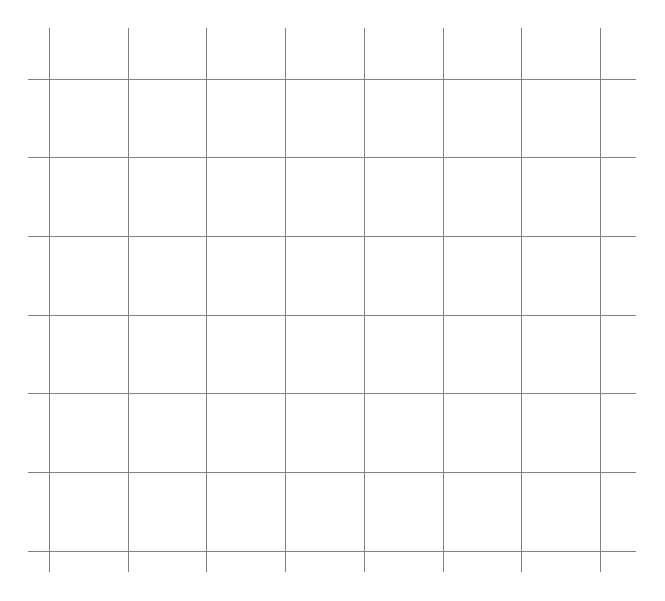
\begin{tikzpicture}[show background grid]
\coordinate (E) at (0,0);
\node (E2) at ($(E)+(100:1)$) {};
\coordinate (F) at (0:4.3);
\node (F2) at ($(F)+(130:1)$) {};
\coordinate (G) at (intersection of E--E2 and F--F2);
\draw (E) coordinate (A)  (F) coordinate (B)   (G) coordinate (C)  ;
\node (U) at  (-3,0) {};
\end{tikzpicture}
}
\\\hline
c)&
\pbox{\linewidth}{
Zeichne die Planfigure und Konstruiere das Dreieck für folgende Werten:\\
$\begin{aligned}
\alpha&=100^\circ \\
c&=4,3~cm\\
\beta&=20^\circ  \\
\end{aligned}$ \\
\tikzstyle{background grid}=[draw, black!15,step=.5cm]
\begin{tikzpicture}[show background grid]
\coordinate (E) at (0,0);
\node (E2) at ($(E)+(100:1)$) {};
\coordinate (F) at (0:4.3);
\node (F2) at ($(F)+(160:1)$) {};
\coordinate (G) at (intersection of E--E2 and F--F2);
\draw (E) coordinate (A)  (F) coordinate (B)   (G) coordinate (C)  ;
\node (U) at  (-3,0) {};
\end{tikzpicture}
}
\\\hline
d)&
\pbox{\linewidth}{
Zeichne die Planfigure und Konstruiere das Dreieck für folgende Werten:\\
$\begin{aligned}
\alpha&=30^\circ \\
b&=5,4~cm\\
\gamma&=30^\circ  \\
\end{aligned}$ \\
\tikzstyle{background grid}=[draw, black!15,step=.5cm]

\begin{tikzpicture}[show background grid]
\coordinate (E) at (0,0);
\node (E2) at ($(E)+(300:1)$) {};
\coordinate (F) at (270:5.4);
\node (F2) at ($(F)+(420:1)$) {};
\coordinate (G) at (intersection of E--E2 and F--F2);
\draw (E) coordinate (C)  (F) coordinate (A)   (G) coordinate (B)  ;
\node (U) at  (-4,-3) {};
\end{tikzpicture}
}
\\\hline
e)&
\pbox{\linewidth}{
Zeichne die Planfigure und Konstruiere das Dreieck für folgende Werten:\\
$\begin{aligned}
\beta&=90^\circ \\
a&=5,7~cm\\
\gamma&=70^\circ  \\
\end{aligned}$ \\
\tikzstyle{background grid}=[draw, black!15,step=.5cm]

\begin{tikzpicture}[show background grid]
\coordinate (E) at (0,0);
\node (E2) at ($(E)+(180:1)$) {};
\coordinate (F) at (90:5.7);
\node (F2) at ($(F)+(200:1)$) {};
\coordinate (G) at (intersection of E--E2 and F--F2);
\draw (E) coordinate (B)  (F) coordinate (C)   (G) coordinate (A)  ;
\node (U) at  (-6,0) {};
\end{tikzpicture}
}
\\\hline
f)&
\pbox{\linewidth}{
Zeichne die Planfigure und Konstruiere das Dreieck für folgende Werten:\\
$\begin{aligned}
\alpha&=70^\circ \\
c&=4~cm\\
\beta&=20^\circ  \\
\end{aligned}$ \\
\tikzstyle{background grid}=[draw, black!15,step=.5cm]
\begin{tikzpicture}[show background grid]
\coordinate (E) at (0,0);
\node (E2) at ($(E)+(70:1)$) {};
\coordinate (F) at (0:4.0);
\node (F2) at ($(F)+(160:1)$) {};
\coordinate (G) at (intersection of E--E2 and F--F2);
\draw (E) coordinate (A)  (F) coordinate (B)   (G) coordinate (C)  ;
\node (U) at  (-3,0) {};
\end{tikzpicture}
}
\\\hline
g)&
\pbox{\linewidth}{
Zeichne die Planfigure und Konstruiere das Dreieck für folgende Werten:\\
$\begin{aligned}
\alpha&=50^\circ \\
c&=4,5~cm\\
\beta&=20^\circ  \\
\end{aligned}$ \\
\tikzstyle{background grid}=[draw, black!15,step=.5cm]
\begin{tikzpicture}[show background grid]
\coordinate (E) at (0,0);
\node (E2) at ($(E)+(50:1)$) {};
\coordinate (F) at (0:4.5);
\node (F2) at ($(F)+(160:1)$) {};
\coordinate (G) at (intersection of E--E2 and F--F2);
\draw (E) coordinate (A)  (F) coordinate (B)   (G) coordinate (C)  ;
\node (U) at  (-3,0) {};
\end{tikzpicture}
}
\\\hline
h)&
\pbox{\linewidth}{
Zeichne die Planfigure und Konstruiere das Dreieck für folgende Werten:\\
$\begin{aligned}
\beta&=110^\circ \\
a&=5,5~cm\\
\gamma&=40^\circ  \\
\end{aligned}$ \\
\tikzstyle{background grid}=[draw, black!15,step=.5cm]

\begin{tikzpicture}[show background grid]
\coordinate (E) at (0,0);
\node (E2) at ($(E)+(200:1)$) {};
\coordinate (F) at (90:5.5);
\node (F2) at ($(F)+(230:1)$) {};
\coordinate (G) at (intersection of E--E2 and F--F2);
\draw (E) coordinate (B)  (F) coordinate (C)   (G) coordinate (A)  ;
\node (U) at  (-6,0) {};
\end{tikzpicture}
}
\\\hline
i)&
\pbox{\linewidth}{
Zeichne die Planfigure und Konstruiere das Dreieck für folgende Werten:\\
$\begin{aligned}
\beta&=20^\circ \\
a&=4,3~cm\\
\gamma&=40^\circ  \\
\end{aligned}$ \\
\tikzstyle{background grid}=[draw, black!15,step=.5cm]
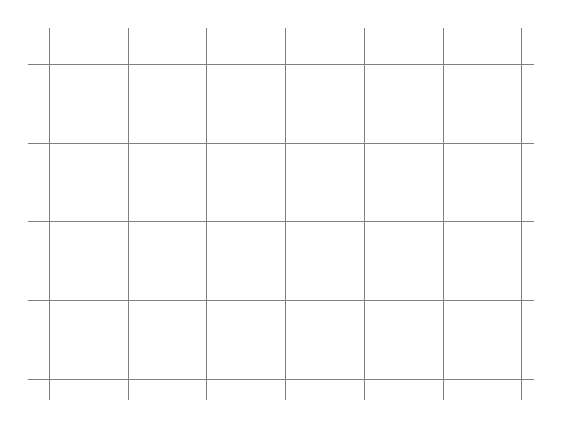
\begin{tikzpicture}[show background grid]
\coordinate (E) at (0,0);
\node (E2) at ($(E)+(110:1)$) {};
\coordinate (F) at (90:4.3);
\node (F2) at ($(F)+(230:1)$) {};
\coordinate (G) at (intersection of E--E2 and F--F2);
\draw (E) coordinate (B)  (F) coordinate (C)   (G) coordinate (A)  ;
\node (U) at  (-6,0) {};
\end{tikzpicture}
}
\\\hline
j)&
\pbox{\linewidth}{
Zeichne die Planfigure und Konstruiere das Dreieck für folgende Werten:\\
$\begin{aligned}
\alpha&=80^\circ \\
b&=4~cm\\
\gamma&=30^\circ  \\
\end{aligned}$ \\
\tikzstyle{background grid}=[draw, black!15,step=.5cm]

\begin{tikzpicture}[show background grid]
\coordinate (E) at (0,0);
\node (E2) at ($(E)+(350:1)$) {};
\coordinate (F) at (270:4.0);
\node (F2) at ($(F)+(420:1)$) {};
\coordinate (G) at (intersection of E--E2 and F--F2);
\draw (E) coordinate (C)  (F) coordinate (A)   (G) coordinate (B)  ;
\node (U) at  (-4,-3) {};
\end{tikzpicture}
}
\\\hline
\end{xltabular}
\vspace{0.5cm}
\newpage
\rightline{Datum: 03.12.2024}
\centerline{{\large Lösungen WSW und SWS}} 
\vspace{0.5cm}

\begin{xltabular}{\textwidth}{|C{0.75cm}|X|}
\arrayrulecolor{black}\hline
a)&
\begin{adjustbox}{max width=15 cm}
\tikzstyle{background grid}=[draw, black!15,step=.5cm]
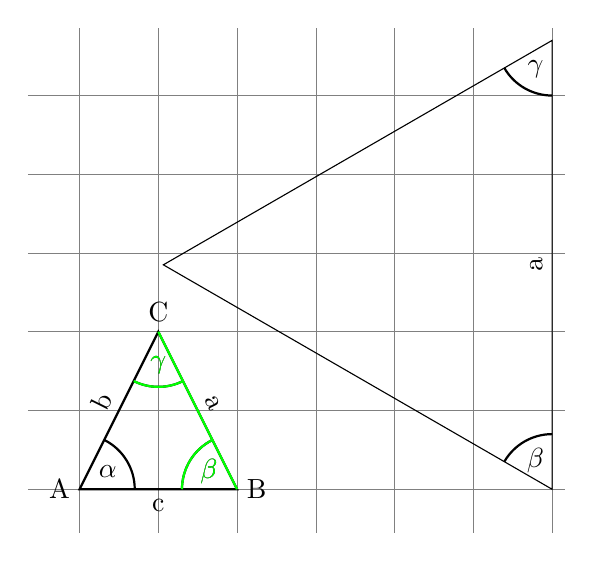
\begin{tikzpicture}[show background grid]
\coordinate (E) at (0,0);
\node (E2) at ($(E)+(150:1)$) {};
\coordinate (F) at (90:5.7);
\node (F2) at ($(F)+(210:1)$) {};
\coordinate (G) at (intersection of E--E2 and F--F2);
\draw (E) coordinate (B)  -- node[above,sloped] {a} (F) coordinate (C)   --  (G) coordinate (A)   --   cycle;
\pic [draw,thick, angle radius=0.7cm, "$\beta$"] {angle = C--B--A};
\pic [draw,thick, angle radius=0.7cm, "$\gamma$"] {angle = A--C--B};
\draw[thick,black] (-6,0) coordinate(A) -- node[below,sloped]{c} ++(2,0) coordinate(B) -- node[above,sloped]{a} ++(-1,2) coordinate(C) -- node[above,sloped]{b} cycle; 
\node[left] at (A) {A};
\node[right] at (B) {B};
\node[above] at (C) {C};
\pic [draw,thick, black,angle radius=0.7cm, "$\alpha$"] {angle = B--A--C};
\pic [draw,thick, black,angle radius=0.7cm, "$\beta$"] {angle = C--B--A};
\pic [draw,thick, black,angle radius=0.7cm, "$\gamma$"] {angle = A--C--B};
\pic [draw,thick, green,angle radius=0.7cm, "$\beta$"] {angle = C--B--A};
\draw[thick,green] (B) -- (C);
\pic [draw,thick, green,angle radius=0.7cm, "$\gamma$"] {angle = A--C--B};
\end{tikzpicture}
\end{adjustbox}
\\\hline
b)&
\begin{adjustbox}{max width=15 cm}
\tikzstyle{background grid}=[draw, black!15,step=.5cm]
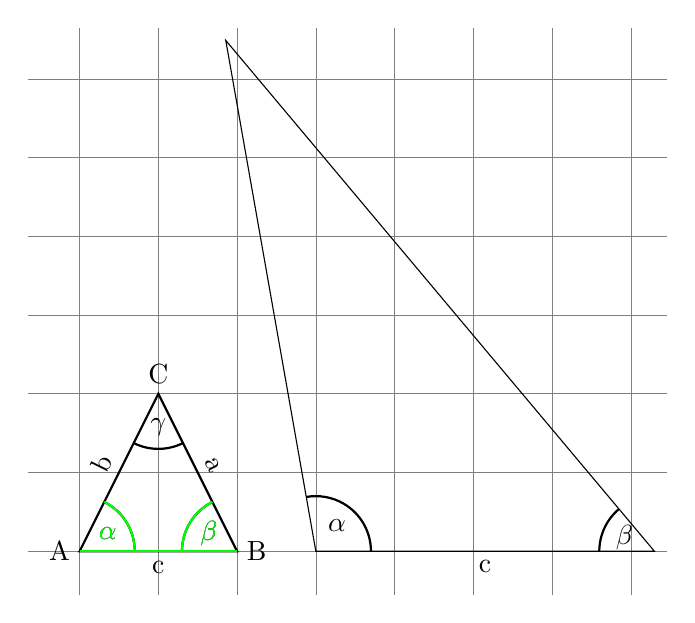
\begin{tikzpicture}[show background grid]
\coordinate (E) at (0,0);
\node (E2) at ($(E)+(100:1)$) {};
\coordinate (F) at (0:4.3);
\node (F2) at ($(F)+(130:1)$) {};
\coordinate (G) at (intersection of E--E2 and F--F2);
\draw (E) coordinate (A)  -- node[below,sloped] {c} (F) coordinate (B)   --  (G) coordinate (C)   --   cycle;
\pic [draw,thick, angle radius=0.7cm, "$\alpha$"] {angle = B--A--C};
\pic [draw,thick, angle radius=0.7cm, "$\beta$"] {angle = C--B--A};
\draw[thick,black] (-3,0) coordinate(A) -- node[below,sloped]{c} ++(2,0) coordinate(B) -- node[above,sloped]{a} ++(-1,2) coordinate(C) -- node[above,sloped]{b} cycle; 
\node[left] at (A) {A};
\node[right] at (B) {B};
\node[above] at (C) {C};
\pic [draw,thick, black,angle radius=0.7cm, "$\alpha$"] {angle = B--A--C};
\pic [draw,thick, black,angle radius=0.7cm, "$\beta$"] {angle = C--B--A};
\pic [draw,thick, black,angle radius=0.7cm, "$\gamma$"] {angle = A--C--B};
\pic [draw,thick, green,angle radius=0.7cm, "$\alpha$"] {angle = B--A--C};
\draw[thick,green] (A) -- (B);
\pic [draw,thick, green,angle radius=0.7cm, "$\beta$"] {angle = C--B--A};
\end{tikzpicture}
\end{adjustbox}
\\\hline
c)&
\begin{adjustbox}{max width=15 cm}
\tikzstyle{background grid}=[draw, black!15,step=.5cm]
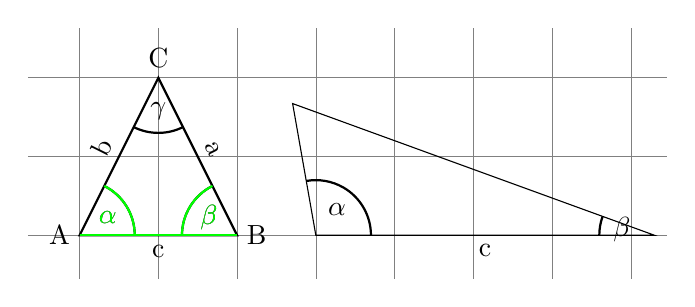
\begin{tikzpicture}[show background grid]
\coordinate (E) at (0,0);
\node (E2) at ($(E)+(100:1)$) {};
\coordinate (F) at (0:4.3);
\node (F2) at ($(F)+(160:1)$) {};
\coordinate (G) at (intersection of E--E2 and F--F2);
\draw (E) coordinate (A)  -- node[below,sloped] {c} (F) coordinate (B)   --  (G) coordinate (C)   --   cycle;
\pic [draw,thick, angle radius=0.7cm, "$\alpha$"] {angle = B--A--C};
\pic [draw,thick, angle radius=0.7cm, "$\beta$"] {angle = C--B--A};
\draw[thick,black] (-3,0) coordinate(A) -- node[below,sloped]{c} ++(2,0) coordinate(B) -- node[above,sloped]{a} ++(-1,2) coordinate(C) -- node[above,sloped]{b} cycle; 
\node[left] at (A) {A};
\node[right] at (B) {B};
\node[above] at (C) {C};
\pic [draw,thick, black,angle radius=0.7cm, "$\alpha$"] {angle = B--A--C};
\pic [draw,thick, black,angle radius=0.7cm, "$\beta$"] {angle = C--B--A};
\pic [draw,thick, black,angle radius=0.7cm, "$\gamma$"] {angle = A--C--B};
\pic [draw,thick, green,angle radius=0.7cm, "$\alpha$"] {angle = B--A--C};
\draw[thick,green] (A) -- (B);
\pic [draw,thick, green,angle radius=0.7cm, "$\beta$"] {angle = C--B--A};
\end{tikzpicture}
\end{adjustbox}
\\\hline
d)&
\begin{adjustbox}{max width=15 cm}
\tikzstyle{background grid}=[draw, black!15,step=.5cm]
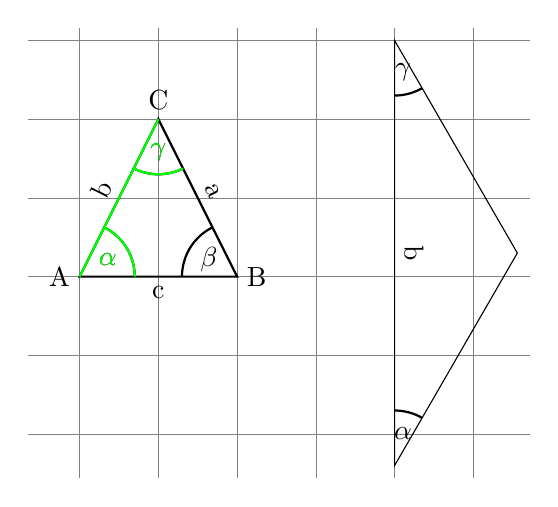
\begin{tikzpicture}[show background grid]
\coordinate (E) at (0,0);
\node (E2) at ($(E)+(300:1)$) {};
\coordinate (F) at (270:5.4);
\node (F2) at ($(F)+(420:1)$) {};
\coordinate (G) at (intersection of E--E2 and F--F2);
\draw (E) coordinate (C)  -- node[above,sloped] {b} (F) coordinate (A)   --  (G) coordinate (B)   --   cycle;
\pic [draw,thick, angle radius=0.7cm, "$\gamma$"] {angle = A--C--B};
\pic [draw,thick, angle radius=0.7cm, "$\alpha$"] {angle = B--A--C};
\draw[thick,black] (-4,-3) coordinate(A) -- node[below,sloped]{c} ++(2,0) coordinate(B) -- node[above,sloped]{a} ++(-1,2) coordinate(C) -- node[above,sloped]{b} cycle; 
\node[left] at (A) {A};
\node[right] at (B) {B};
\node[above] at (C) {C};
\pic [draw,thick, black,angle radius=0.7cm, "$\alpha$"] {angle = B--A--C};
\pic [draw,thick, black,angle radius=0.7cm, "$\beta$"] {angle = C--B--A};
\pic [draw,thick, black,angle radius=0.7cm, "$\gamma$"] {angle = A--C--B};
\pic [draw,thick, green,angle radius=0.7cm, "$\gamma$"] {angle = A--C--B};
\draw[thick,green] (A) -- (C);
\pic [draw,thick, green,angle radius=0.7cm, "$\alpha$"] {angle = B--A--C};
\end{tikzpicture}
\end{adjustbox}
\\\hline
e)&
\begin{adjustbox}{max width=15 cm}
\tikzstyle{background grid}=[draw, black!15,step=.5cm]
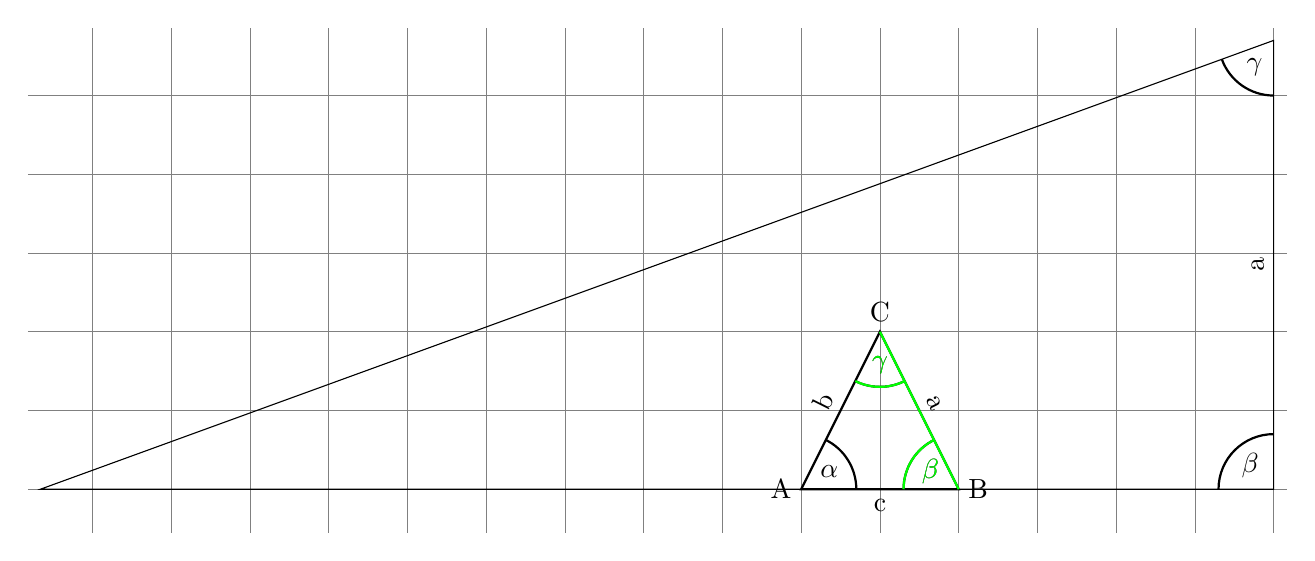
\begin{tikzpicture}[show background grid]
\coordinate (E) at (0,0);
\node (E2) at ($(E)+(180:1)$) {};
\coordinate (F) at (90:5.7);
\node (F2) at ($(F)+(200:1)$) {};
\coordinate (G) at (intersection of E--E2 and F--F2);
\draw (E) coordinate (B)  -- node[above,sloped] {a} (F) coordinate (C)   --  (G) coordinate (A)   --   cycle;
\pic [draw,thick, angle radius=0.7cm, "$\beta$"] {angle = C--B--A};
\pic [draw,thick, angle radius=0.7cm, "$\gamma$"] {angle = A--C--B};
\draw[thick,black] (-6,0) coordinate(A) -- node[below,sloped]{c} ++(2,0) coordinate(B) -- node[above,sloped]{a} ++(-1,2) coordinate(C) -- node[above,sloped]{b} cycle; 
\node[left] at (A) {A};
\node[right] at (B) {B};
\node[above] at (C) {C};
\pic [draw,thick, black,angle radius=0.7cm, "$\alpha$"] {angle = B--A--C};
\pic [draw,thick, black,angle radius=0.7cm, "$\beta$"] {angle = C--B--A};
\pic [draw,thick, black,angle radius=0.7cm, "$\gamma$"] {angle = A--C--B};
\pic [draw,thick, green,angle radius=0.7cm, "$\beta$"] {angle = C--B--A};
\draw[thick,green] (B) -- (C);
\pic [draw,thick, green,angle radius=0.7cm, "$\gamma$"] {angle = A--C--B};
\end{tikzpicture}
\end{adjustbox}
\\\hline
f)&
\begin{adjustbox}{max width=15 cm}
\tikzstyle{background grid}=[draw, black!15,step=.5cm]
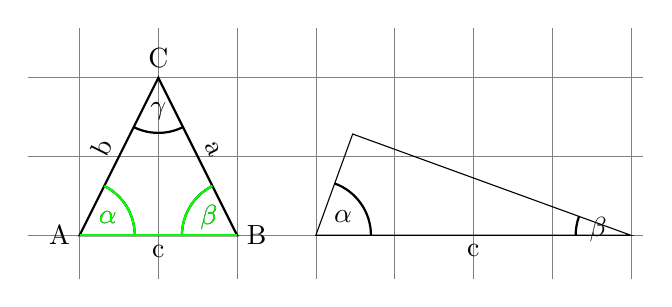
\begin{tikzpicture}[show background grid]
\coordinate (E) at (0,0);
\node (E2) at ($(E)+(70:1)$) {};
\coordinate (F) at (0:4.0);
\node (F2) at ($(F)+(160:1)$) {};
\coordinate (G) at (intersection of E--E2 and F--F2);
\draw (E) coordinate (A)  -- node[below,sloped] {c} (F) coordinate (B)   --  (G) coordinate (C)   --   cycle;
\pic [draw,thick, angle radius=0.7cm, "$\alpha$"] {angle = B--A--C};
\pic [draw,thick, angle radius=0.7cm, "$\beta$"] {angle = C--B--A};
\draw[thick,black] (-3,0) coordinate(A) -- node[below,sloped]{c} ++(2,0) coordinate(B) -- node[above,sloped]{a} ++(-1,2) coordinate(C) -- node[above,sloped]{b} cycle; 
\node[left] at (A) {A};
\node[right] at (B) {B};
\node[above] at (C) {C};
\pic [draw,thick, black,angle radius=0.7cm, "$\alpha$"] {angle = B--A--C};
\pic [draw,thick, black,angle radius=0.7cm, "$\beta$"] {angle = C--B--A};
\pic [draw,thick, black,angle radius=0.7cm, "$\gamma$"] {angle = A--C--B};
\pic [draw,thick, green,angle radius=0.7cm, "$\alpha$"] {angle = B--A--C};
\draw[thick,green] (A) -- (B);
\pic [draw,thick, green,angle radius=0.7cm, "$\beta$"] {angle = C--B--A};
\end{tikzpicture}
\end{adjustbox}
\\\hline
g)&
\begin{adjustbox}{max width=15 cm}
\tikzstyle{background grid}=[draw, black!15,step=.5cm]
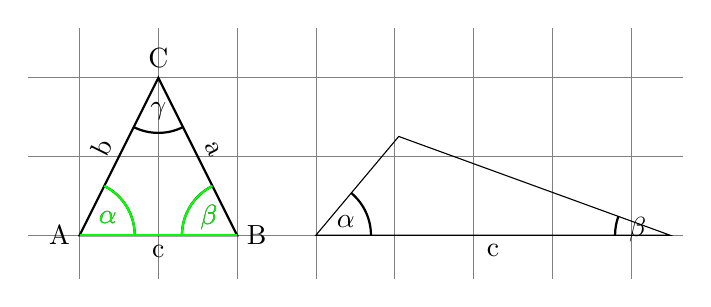
\begin{tikzpicture}[show background grid]
\coordinate (E) at (0,0);
\node (E2) at ($(E)+(50:1)$) {};
\coordinate (F) at (0:4.5);
\node (F2) at ($(F)+(160:1)$) {};
\coordinate (G) at (intersection of E--E2 and F--F2);
\draw (E) coordinate (A)  -- node[below,sloped] {c} (F) coordinate (B)   --  (G) coordinate (C)   --   cycle;
\pic [draw,thick, angle radius=0.7cm, "$\alpha$"] {angle = B--A--C};
\pic [draw,thick, angle radius=0.7cm, "$\beta$"] {angle = C--B--A};
\draw[thick,black] (-3,0) coordinate(A) -- node[below,sloped]{c} ++(2,0) coordinate(B) -- node[above,sloped]{a} ++(-1,2) coordinate(C) -- node[above,sloped]{b} cycle; 
\node[left] at (A) {A};
\node[right] at (B) {B};
\node[above] at (C) {C};
\pic [draw,thick, black,angle radius=0.7cm, "$\alpha$"] {angle = B--A--C};
\pic [draw,thick, black,angle radius=0.7cm, "$\beta$"] {angle = C--B--A};
\pic [draw,thick, black,angle radius=0.7cm, "$\gamma$"] {angle = A--C--B};
\pic [draw,thick, green,angle radius=0.7cm, "$\alpha$"] {angle = B--A--C};
\draw[thick,green] (A) -- (B);
\pic [draw,thick, green,angle radius=0.7cm, "$\beta$"] {angle = C--B--A};
\end{tikzpicture}
\end{adjustbox}
\\\hline
h)&
\begin{adjustbox}{max width=15 cm}
\tikzstyle{background grid}=[draw, black!15,step=.5cm]
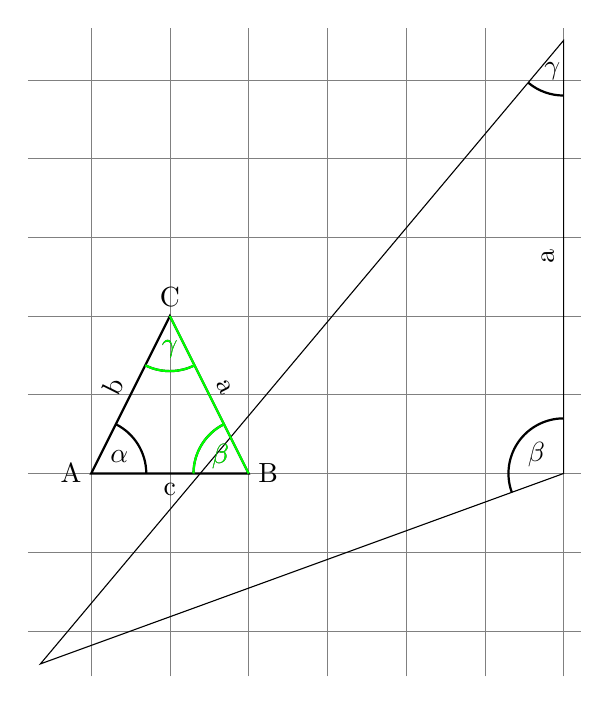
\begin{tikzpicture}[show background grid]
\coordinate (E) at (0,0);
\node (E2) at ($(E)+(200:1)$) {};
\coordinate (F) at (90:5.5);
\node (F2) at ($(F)+(230:1)$) {};
\coordinate (G) at (intersection of E--E2 and F--F2);
\draw (E) coordinate (B)  -- node[above,sloped] {a} (F) coordinate (C)   --  (G) coordinate (A)   --   cycle;
\pic [draw,thick, angle radius=0.7cm, "$\beta$"] {angle = C--B--A};
\pic [draw,thick, angle radius=0.7cm, "$\gamma$"] {angle = A--C--B};
\draw[thick,black] (-6,0) coordinate(A) -- node[below,sloped]{c} ++(2,0) coordinate(B) -- node[above,sloped]{a} ++(-1,2) coordinate(C) -- node[above,sloped]{b} cycle; 
\node[left] at (A) {A};
\node[right] at (B) {B};
\node[above] at (C) {C};
\pic [draw,thick, black,angle radius=0.7cm, "$\alpha$"] {angle = B--A--C};
\pic [draw,thick, black,angle radius=0.7cm, "$\beta$"] {angle = C--B--A};
\pic [draw,thick, black,angle radius=0.7cm, "$\gamma$"] {angle = A--C--B};
\pic [draw,thick, green,angle radius=0.7cm, "$\beta$"] {angle = C--B--A};
\draw[thick,green] (B) -- (C);
\pic [draw,thick, green,angle radius=0.7cm, "$\gamma$"] {angle = A--C--B};
\end{tikzpicture}
\end{adjustbox}
\\\hline
i)&
\begin{adjustbox}{max width=15 cm}
\tikzstyle{background grid}=[draw, black!15,step=.5cm]
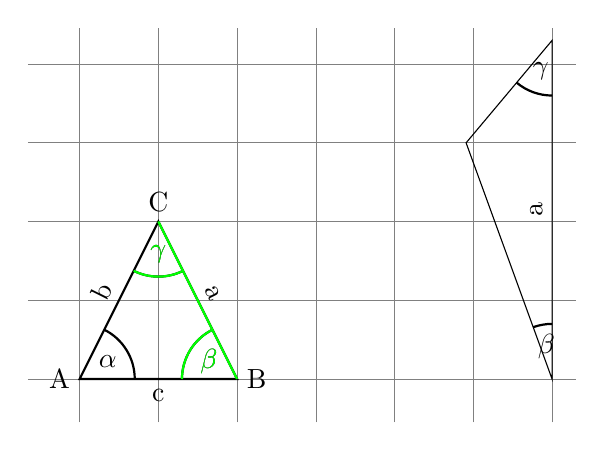
\begin{tikzpicture}[show background grid]
\coordinate (E) at (0,0);
\node (E2) at ($(E)+(110:1)$) {};
\coordinate (F) at (90:4.3);
\node (F2) at ($(F)+(230:1)$) {};
\coordinate (G) at (intersection of E--E2 and F--F2);
\draw (E) coordinate (B)  -- node[above,sloped] {a} (F) coordinate (C)   --  (G) coordinate (A)   --   cycle;
\pic [draw,thick, angle radius=0.7cm, "$\beta$"] {angle = C--B--A};
\pic [draw,thick, angle radius=0.7cm, "$\gamma$"] {angle = A--C--B};
\draw[thick,black] (-6,0) coordinate(A) -- node[below,sloped]{c} ++(2,0) coordinate(B) -- node[above,sloped]{a} ++(-1,2) coordinate(C) -- node[above,sloped]{b} cycle; 
\node[left] at (A) {A};
\node[right] at (B) {B};
\node[above] at (C) {C};
\pic [draw,thick, black,angle radius=0.7cm, "$\alpha$"] {angle = B--A--C};
\pic [draw,thick, black,angle radius=0.7cm, "$\beta$"] {angle = C--B--A};
\pic [draw,thick, black,angle radius=0.7cm, "$\gamma$"] {angle = A--C--B};
\pic [draw,thick, green,angle radius=0.7cm, "$\beta$"] {angle = C--B--A};
\draw[thick,green] (B) -- (C);
\pic [draw,thick, green,angle radius=0.7cm, "$\gamma$"] {angle = A--C--B};
\end{tikzpicture}
\end{adjustbox}
\\\hline
j)&
\begin{adjustbox}{max width=15 cm}
\tikzstyle{background grid}=[draw, black!15,step=.5cm]
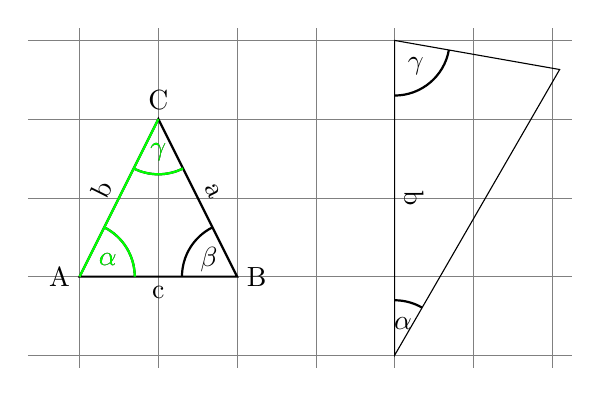
\begin{tikzpicture}[show background grid]
\coordinate (E) at (0,0);
\node (E2) at ($(E)+(350:1)$) {};
\coordinate (F) at (270:4.0);
\node (F2) at ($(F)+(420:1)$) {};
\coordinate (G) at (intersection of E--E2 and F--F2);
\draw (E) coordinate (C)  -- node[above,sloped] {b} (F) coordinate (A)   --  (G) coordinate (B)   --   cycle;
\pic [draw,thick, angle radius=0.7cm, "$\gamma$"] {angle = A--C--B};
\pic [draw,thick, angle radius=0.7cm, "$\alpha$"] {angle = B--A--C};
\draw[thick,black] (-4,-3) coordinate(A) -- node[below,sloped]{c} ++(2,0) coordinate(B) -- node[above,sloped]{a} ++(-1,2) coordinate(C) -- node[above,sloped]{b} cycle; 
\node[left] at (A) {A};
\node[right] at (B) {B};
\node[above] at (C) {C};
\pic [draw,thick, black,angle radius=0.7cm, "$\alpha$"] {angle = B--A--C};
\pic [draw,thick, black,angle radius=0.7cm, "$\beta$"] {angle = C--B--A};
\pic [draw,thick, black,angle radius=0.7cm, "$\gamma$"] {angle = A--C--B};
\pic [draw,thick, green,angle radius=0.7cm, "$\gamma$"] {angle = A--C--B};
\draw[thick,green] (A) -- (C);
\pic [draw,thick, green,angle radius=0.7cm, "$\alpha$"] {angle = B--A--C};
\end{tikzpicture}
\end{adjustbox}
\\\hline
\end{xltabular}
\vspace{0.5cm}
\end{document}